% !TEX spellcheck = en_US

\documentclass[10pt,journal,compsoc]{IEEEtran}

%\usepackage{cite}
%\usepackage[caption=false,font=footnotesize]{subfig}
%\usepackage{url}





%: ~~~~~~~~~~~~~~~~~~~~~~~~~~~~~~~~~~~~~~~ V HB Packages v2020-12-11
	\usepackage[utf8]{inputenc} % To use Unicode characters
	\usepackage[iso]{datetime}
	\newcommand{\hbTimeStamp}{{\color{red}--Draft-- v\today/\currenttime}} % version
	%	\usepackage{etex}
	\usepackage{amssymb}
	\usepackage{enumitem}
	
	\usepackage[a4paper]{geometry}
	
	\usepackage{xcolor}
	% black, blue, brown, cyan, darkgray, gray, green, lightgray, lime, 
	% magenta, olive, orange, pink, purple, red, teal, violet, white, yellow
		\definecolor{darkred}{rgb}{0.8,0.1,0.1}
		\definecolor{darkgreen}{rgb}{0,0.5,0}
		\definecolor{darkblue}{rgb}{0,0,0.5}
		\colorlet{RED}{red}

	\usepackage[colorlinks=true,linkcolor=red,urlcolor=blue,citecolor=red]%
		{hyperref}
	\usepackage{graphicx,epstopdf}
	% \graphicspath{{fig}}
	\graphicspath{{../common/figures/}}
	% \DeclareGraphicsExtensions{.pdf,.jpeg,.png,.eps}
	% \DeclareGraphicsRule{.tif}{png}{.png}%
	%	{`convert #1 `dirname #1`/`basename #1 .tif`.png}
%	\usepackage{subfigure}
%	\usepackage{subfig}
	\usepackage{subcaption}
% ~~~~~~~~~~~~~~~~~~~~~~~~~~~~~~~~~~~~~~~ A




%: ~~~~~~~~~~~~~~~~~~~~~~~~~~~~~~~~~~~~~~~ V HB Math v2020-11-21
	\usepackage{amsmath, amssymb,amsfonts,amsthm}
	\newcommand{\hDefined}[1]{\textcolor{darkred}{\textit{#1}}}	
	\newcommand{\hVec}[1]{\mathbf{#1}}	 
	\newcommand{\hAbs}[1]{\ensuremath{\left \lvert \, #1 \, \right \rvert} } % |x|
	\newcommand{\hMat}[1]{\mathbf{#1}}
	\newcommand{\hArgmin}[2]{\underset{#1}{\operatorname{arg \, min}}\;#2}
	\newcommand{\hArgmax}[2]{\underset{#1}{\operatorname{arg \, max}}\;#2}
	%
	\theoremstyle{plain}
	\newtheorem{thm}{Theorem}[section]
	\newtheorem{lem}[thm]{Lemma}
	\newtheorem{prop}[thm]{Proposition}
	\newtheorem*{cor}{Corollary}
	\theoremstyle{definition}
	\newtheorem{defn}{Definition}[section]
	\newtheorem{conj}{Conjecture}[section]
	\newtheorem{exmp}{Example}[section]
	\theoremstyle{remark}
	\newtheorem*{rem}{Remark}
	\newtheorem*{note}{Note}
% ~~~~~~~~~~~~~~~~~~~~~~~~~~~~~~~~~~~~~~~ A




%: ~~~~~~~~~~~~~~~~~~~~~~~~~~~~~~~~~~~~~~~ V HB Common Declarations v20200421
	\newcommand{\reffig}[1]{Fig.~\ref{#1}}
	\newcommand{\refeq}[1]{Eq.~\ref{#1}}
	\newcommand{\reftbl}[1]{Table~\ref{#1}}
	\newcommand{\refsec}[1]{Sec.~\ref{#1}}
	\newcommand{\refcite}[1]{Ref~\cite{#1}}
	\newcommand{\refalg}[1]{Algorithm~\ref{#1}}
	\newcommand{\reflst}[1]{List.~\ref{#1}}  % code listing
	%
	\newcommand{\refthm}[1]{Theorem~\ref{#1}}
	\newcommand{\refthmA}[2]{\refthm{#1}(\ref{#2}}
	\newcommand{\reflem}[1]{Lemma~\ref{#1}}
	\newcommand{\refdef}[1]{Definition~\ref{#1}}
	\newcommand{\refexmp}[1]{Example~\ref{#1}}
	%
	\newcommand{\hbQuote}[1]{{\small \textsf{``#1''}}}
	%
	\newcommand{\hbCode}[1]{\texttt{#1}}
	%
	\newcommand{\hbIdea}[1]{{\color{olive}{\scriptsize [{#1}]}}}
	\newcommand{\hbFootnote}[2]{\footnote{{\color{red} @#1 : }#2}}
% ~~~~~~~~~~~~~~~~~~~~~~~~~~~~~~~~~~~~~~~ A





\hyphenation{
	op-tical net-works semi-conduc-tor
}


\begin{document}
\title{
	Title of the paper
}

\author{
	YourName~Lastname,
	Haluk~O.~Bingol
	\IEEEcompsocitemizethanks{
		\IEEEcompsocthanksitem Y. Lastname and H. O. Bingol  are with Bogazici University.
	}%
%	\thanks{
%		Manuscript received April 19, 2005; 
%		revised August 26, 2015.
%	}%
}


\markboth{
	\hbTimeStamp
}%
{
	\hbTimeStamp
}

\IEEEtitleabstractindextext{%
	\begin{abstract}
		The abstract goes here.
	\end{abstract}
	
	\begin{IEEEkeywords}
		KeywordA, keywordB.
	\end{IEEEkeywords}
}

\maketitle




% ~~~~~~~~~~~~~~~~~~~~~~~~~~~~~~~~~~~~~~
\section{Helper for \LaTeX| Usage}

Please read 
\href
	{https://github.com/halukbingol/LaTeX-Templates/tree/master/bingol-StudentDirectory/0readme}
	{https://github.com/halukbingol/LaTeX-Templates/tree/master/bingol-StudentDirectory/0readme}
for better \LaTeX\ usage.

In short
\begin{itemize}
	
	\item 
	Try to use shorter lines.
	
	\item 
	Sample of how to cite~\cite{%
		chomsky1993,
		wikiComplexNetwork%
		}.
	Bib file is defined at the end of this file with\\
	\texttt{bibliographystyle{IEEEtran}} and\\
	\texttt{bibliography{pCovid-v2}}.\\
	Requires four compilations 
	(i)~LaTeX, 
	(ii)~BibTex, 
	(iii)~LaTeX, and  
	(iv)~LaTeX.
	
	\item 
	Sample of how to reference a figure \reffig{fig:figureA}.
	Requires two compilations 
	(i)~LaTeX, 
	(ii)~LaTeX.
	
	\item 
	Sample of how to reference an equation \refeq{eq:bbb}.
	Requires two compilations 
	(i)~LaTeX, 
	(ii)~LaTeX.
	
\end{itemize}






\begin{figure}[htbp]
\begin{center}
	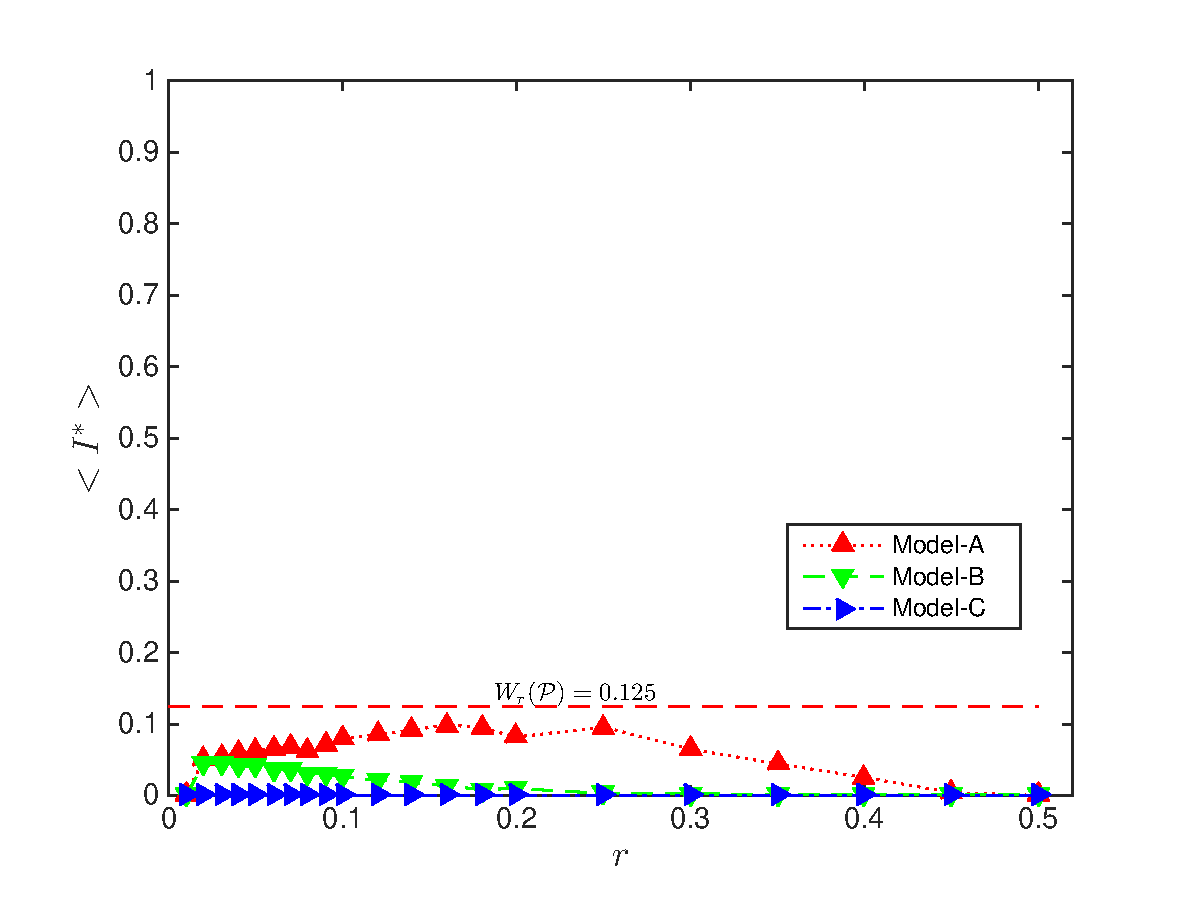
\includegraphics[width=\columnwidth]
		{Fig-FigureA}
	\caption{Houlsehold layer.}
	\label{fig:figureA}
\end{center}
\end{figure}

\begin{align}
	x = y
	\label{eq:bbb}
\end{align}




% ~~~~~~~~~~~~~~~~~~~~~~~~~~~~~~~~~~~~~~
\section{Network}




\section*{Acknowledgment}

The authors would like to thank Aaaa.
%
This work is partially supported by 
the Turkish Directorate of Strategy and Budget
under the TAM Project number 2007K12-873.


\bibliographystyle{IEEEtran}
\bibliography{bingol-template-paper}


\end{document}


